\documentclass[10pt,a4paper,noindentfirst]{article}\usepackage[]{graphicx}\usepackage[]{color}
%% maxwidth is the original width if it is less than linewidth
%% otherwise use linewidth (to make sure the graphics do not exceed the margin)
\makeatletter
\def\maxwidth{ %
  \ifdim\Gin@nat@width>\linewidth
    \linewidth
  \else
    \Gin@nat@width
  \fi
}
\makeatother

\definecolor{fgcolor}{rgb}{0.345, 0.345, 0.345}
\newcommand{\hlnum}[1]{\textcolor[rgb]{0.686,0.059,0.569}{#1}}%
\newcommand{\hlstr}[1]{\textcolor[rgb]{0.192,0.494,0.8}{#1}}%
\newcommand{\hlcom}[1]{\textcolor[rgb]{0.678,0.584,0.686}{\textit{#1}}}%
\newcommand{\hlopt}[1]{\textcolor[rgb]{0,0,0}{#1}}%
\newcommand{\hlstd}[1]{\textcolor[rgb]{0.345,0.345,0.345}{#1}}%
\newcommand{\hlkwa}[1]{\textcolor[rgb]{0.161,0.373,0.58}{\textbf{#1}}}%
\newcommand{\hlkwb}[1]{\textcolor[rgb]{0.69,0.353,0.396}{#1}}%
\newcommand{\hlkwc}[1]{\textcolor[rgb]{0.333,0.667,0.333}{#1}}%
\newcommand{\hlkwd}[1]{\textcolor[rgb]{0.737,0.353,0.396}{\textbf{#1}}}%

\usepackage{framed}
\makeatletter
\newenvironment{kframe}{%
 \def\at@end@of@kframe{}%
 \ifinner\ifhmode%
  \def\at@end@of@kframe{\end{minipage}}%
  \begin{minipage}{\columnwidth}%
 \fi\fi%
 \def\FrameCommand##1{\hskip\@totalleftmargin \hskip-\fboxsep
 \colorbox{shadecolor}{##1}\hskip-\fboxsep
     % There is no \\@totalrightmargin, so:
     \hskip-\linewidth \hskip-\@totalleftmargin \hskip\columnwidth}%
 \MakeFramed {\advance\hsize-\width
   \@totalleftmargin\z@ \linewidth\hsize
   \@setminipage}}%
 {\par\unskip\endMakeFramed%
 \at@end@of@kframe}
\makeatother

\definecolor{shadecolor}{rgb}{.97, .97, .97}
\definecolor{messagecolor}{rgb}{0, 0, 0}
\definecolor{warningcolor}{rgb}{1, 0, 1}
\definecolor{errorcolor}{rgb}{1, 0, 0}
\newenvironment{knitrout}{}{} % an empty environment to be redefined in TeX

\usepackage{alltt}

\usepackage[T1]{fontenc}
\usepackage[polish]{babel}
\usepackage[cp1250]{inputenc}
\usepackage{amsmath}
\usepackage{amsfonts}
\usepackage{graphicx}
\usepackage{setspace}
\usepackage{savesym}
\savesymbol{arc}
\usepackage{color}
\usepackage{xcolor}
\usepackage{pict2e}
\usepackage{epstopdf}
\usepackage{geometry}

\newgeometry{tmargin=0.9cm, bmargin=0.9cm, lmargin=0.9cm, rmargin=0.9cm}
\pagestyle{empty}
\linespread{1.2}
\IfFileExists{upquote.sty}{\usepackage{upquote}}{}
\begin{document}

\begin{knitrout}
\definecolor{shadecolor}{rgb}{0.969, 0.969, 0.969}\color{fgcolor}\begin{kframe}
\begin{alltt}
\hlcom{# zad.1}

\hlstd{sz} \hlkwb{<-} \hlkwd{read.table}\hlstd{(}\hlstr{"http://gamma.mini.pw.edu.pl/~szymanowskih/lab5/szereg.txt"}\hlstd{)}
\hlstd{sz} \hlkwb{<-} \hlkwd{as.numeric}\hlstd{(sz[,}\hlnum{1}\hlstd{])}
\hlkwd{head}\hlstd{(sz)}
\end{alltt}
\begin{verbatim}
## [1] -180.748  -37.494  240.327 -200.448    7.833  285.570
\end{verbatim}
\begin{alltt}
\hlkwd{ts.plot}\hlstd{(sz)}
\end{alltt}
\end{kframe}

{\centering \includegraphics[width=\maxwidth]{figure/unnamed-chunk-11} 

}


\begin{kframe}\begin{alltt}
\hlstd{n} \hlkwb{<-} \hlkwd{length}\hlstd{(sz)}

\hlcom{# pierwszy sposob - roznicowanie:}

\hlstd{szd} \hlkwb{<-} \hlkwd{diff}\hlstd{(sz)}   \hlcom{# zmienia sie rzad szeregu MA!!!}
\hlkwd{ts.plot}\hlstd{(szd)}
\end{alltt}
\end{kframe}

{\centering 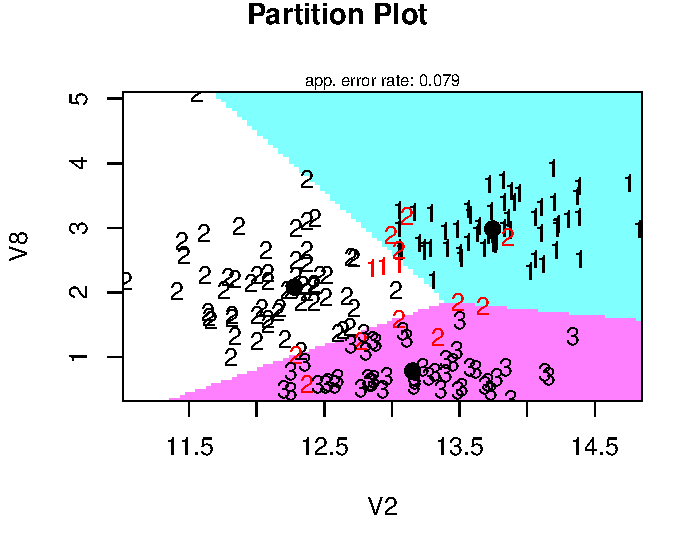
\includegraphics[width=\maxwidth]{figure/unnamed-chunk-12} 

}


\begin{kframe}\begin{alltt}
\hlstd{mod1} \hlkwb{<-} \hlkwd{arima}\hlstd{(szd,}\hlkwd{c}\hlstd{(}\hlnum{1}\hlstd{,}\hlnum{0}\hlstd{,}\hlnum{3}\hlstd{),}\hlkwc{method}\hlstd{=}\hlstr{"ML"}\hlstd{,}\hlkwc{include.mean}\hlstd{=}\hlnum{TRUE}\hlstd{)}

\hlstd{phi1} \hlkwb{<-} \hlstd{mod1}\hlopt{$}\hlstd{coef[}\hlnum{1}\hlstd{]}
\hlstd{theta1} \hlkwb{<-} \hlstd{mod1}\hlopt{$}\hlstd{coef[}\hlnum{2}\hlstd{]}\hlopt{+}\hlnum{1}
\hlstd{theta2} \hlkwb{<-} \hlopt{-}\hlstd{mod1}\hlopt{$}\hlstd{coef[}\hlnum{4}\hlstd{]}
\hlstd{a} \hlkwb{<-} \hlstd{mod1}\hlopt{$}\hlstd{coef[}\hlnum{5}\hlstd{]}

\hlcom{# b - tak mozemy je odzyskac:}

\hlstd{ut} \hlkwb{<-} \hlstd{sz}\hlopt{-}\hlstd{(}\hlnum{1}\hlopt{:}\hlstd{n)}\hlopt{*}\hlstd{a}
\hlstd{b} \hlkwb{<-} \hlkwd{mean}\hlstd{(ut)}

\hlstd{par} \hlkwb{<-} \hlkwd{c}\hlstd{(phi1,theta1,theta2,a,b)}
\hlkwd{names}\hlstd{(par)} \hlkwb{<-} \hlkwd{c}\hlstd{(}\hlstr{"phi1"}\hlstd{,}\hlstr{"theta1"}\hlstd{,}\hlstr{"theta2"}\hlstd{,}\hlstr{"a"}\hlstd{,}\hlstr{"b"}\hlstd{)}
\hlstd{par}
\end{alltt}
\begin{verbatim}
##    phi1  theta1  theta2       a       b 
## -0.7400 -0.2884  0.5300  1.9930  0.8702
\end{verbatim}
\begin{alltt}
\hlcom{# drugi sposob - dopasowanie modelu:}

\hlstd{l} \hlkwb{<-} \hlkwd{lm}\hlstd{(sz}\hlopt{~}\hlkwd{c}\hlstd{(}\hlnum{1}\hlopt{:}\hlstd{n))}
\hlkwd{summary}\hlstd{(l)}
\end{alltt}
\begin{verbatim}
## 
## Call:
## lm(formula = sz ~ c(1:n))
## 
## Residuals:
##     Min      1Q  Median      3Q     Max 
## -2728.0  -480.9     0.2   486.9  2424.6 
## 
## Coefficients:
##             Estimate Std. Error t value Pr(>|t|)    
## (Intercept)   1.3527    44.3859    0.03     0.98    
## c(1:n)        1.9920     0.0768   25.93   <2e-16 ***
## ---
## Signif. codes:  0 '***' 0.001 '**' 0.01 '*' 0.05 '.' 0.1 ' ' 1
## 
## Residual standard error: 701 on 998 degrees of freedom
## Multiple R-squared:  0.403,	Adjusted R-squared:  0.402 
## F-statistic:  672 on 1 and 998 DF,  p-value: <2e-16
\end{verbatim}
\begin{alltt}
\hlstd{ut} \hlkwb{<-} \hlstd{sz} \hlopt{-} \hlstd{l}\hlopt{$}\hlstd{coef[}\hlnum{1}\hlstd{]}\hlopt{-}\hlstd{l}\hlopt{$}\hlstd{coef[}\hlnum{2}\hlstd{]}\hlopt{*}\hlstd{(}\hlnum{1}\hlopt{:}\hlstd{n)}

\hlstd{mod2} \hlkwb{<-} \hlkwd{arima}\hlstd{(ut,}\hlkwd{c}\hlstd{(}\hlnum{1}\hlstd{,}\hlnum{0}\hlstd{,}\hlnum{2}\hlstd{),}\hlkwc{method}\hlstd{=}\hlstr{"ML"}\hlstd{,}\hlkwc{include.mean}\hlstd{=}\hlnum{FALSE}\hlstd{)}
\hlcom{# dlaczego bez sredniej? Bo byla juz uwzgledniona wczesniej!}

\hlstd{par2} \hlkwb{<-} \hlkwd{c}\hlstd{(mod2}\hlopt{$}\hlstd{coef,l}\hlopt{$}\hlstd{coef[}\hlnum{2}\hlopt{:}\hlnum{1}\hlstd{])}
\hlkwd{names}\hlstd{(par2)} \hlkwb{<-} \hlkwd{c}\hlstd{(}\hlstr{"phi1"}\hlstd{,}\hlstr{"theta1"}\hlstd{,}\hlstr{"theta2"}\hlstd{,}\hlstr{"a"}\hlstd{,}\hlstr{"b"}\hlstd{)}

\hlstd{par}
\end{alltt}
\begin{verbatim}
##    phi1  theta1  theta2       a       b 
## -0.7400 -0.2884  0.5300  1.9930  0.8702
\end{verbatim}
\begin{alltt}
\hlstd{par2}    \hlcom{# oprocz interceptu wyszlo podobnie :D}
\end{alltt}
\begin{verbatim}
##    phi1  theta1  theta2       a       b 
## -0.7403 -0.2888  0.5293  1.9920  1.3527
\end{verbatim}
\begin{alltt}
\hlcom{# prawdziwa wartosc: c(-3/4,-1/3,1/2,5)  -> tak byly generowane te dane}
\hlcom{# wyraz wolny ogolnie sie bardzo slabo estymuje...}

\hlcom{# zad.2}

\hlstd{lac} \hlkwb{<-} \hlkwd{read.table}\hlstd{(}\hlstr{"http://gamma.mini.pw.edu.pl/~szymanowskih/lab5/LACounty.txt"}\hlstd{,}\hlkwc{header}\hlstd{=}\hlnum{TRUE}\hlstd{)}
\hlkwd{head}\hlstd{(lac,}\hlnum{2}\hlstd{)}
\end{alltt}
\begin{verbatim}
##   DATE  TEMP  PART CARDIO
## 1    1 72.38 72.72  97.85
## 2    2 67.19 49.60 104.64
\end{verbatim}
\begin{alltt}
\hlcom{# a)}

\hlkwd{plot}\hlstd{(lac}\hlopt{$}\hlstd{TEMP,lac}\hlopt{$}\hlstd{CARDIO)}
\hlcom{# widac, ze w miare ukladaja sie na paraboli, }
\hlcom{# wiec wprowadzmy nowa zmienna kwadrawowa:}

\hlstd{t} \hlkwb{<-} \hlstd{lac}\hlopt{$}\hlstd{DATE}
\hlstd{y} \hlkwb{<-} \hlstd{lac}\hlopt{$}\hlstd{CARDIO}
\hlstd{t1} \hlkwb{<-} \hlstd{lac}\hlopt{$}\hlstd{TEMP} \hlopt{-} \hlkwd{mean}\hlstd{(lac}\hlopt{$}\hlstd{TEMP)}
\hlstd{t2} \hlkwb{<-} \hlstd{(lac}\hlopt{$}\hlstd{TEMP} \hlopt{-} \hlkwd{mean}\hlstd{(lac}\hlopt{$}\hlstd{TEMP))}\hlopt{^}\hlnum{2}
\hlstd{p} \hlkwb{<-} \hlstd{lac}\hlopt{$}\hlstd{PART}

\hlcom{# b)}

\hlstd{mod1} \hlkwb{<-} \hlkwd{lm}\hlstd{(y}\hlopt{~}\hlstd{t}\hlopt{+}\hlstd{t1}\hlopt{+}\hlstd{t2}\hlopt{+}\hlstd{p)}
\hlkwd{summary}\hlstd{(mod1)}
\end{alltt}
\begin{verbatim}
## 
## Call:
## lm(formula = y ~ t + t1 + t2 + p)
## 
## Residuals:
##     Min      1Q  Median      3Q     Max 
## -19.076  -4.215  -0.488   3.744  29.245 
## 
## Coefficients:
##             Estimate Std. Error t value Pr(>|t|)    
## (Intercept) 81.59224    1.10215   74.03  < 2e-16 ***
## t           -0.02684    0.00194  -13.82  < 2e-16 ***
## t1          -0.47247    0.03162  -14.94  < 2e-16 ***
## t2           0.02259    0.00283    7.99  9.3e-15 ***
## p            0.25535    0.01886   13.54  < 2e-16 ***
## ---
## Signif. codes:  0 '***' 0.001 '**' 0.01 '*' 0.05 '.' 0.1 ' ' 1
## 
## Residual standard error: 6.39 on 503 degrees of freedom
## Multiple R-squared:  0.595,	Adjusted R-squared:  0.592 
## F-statistic:  185 on 4 and 503 DF,  p-value: <2e-16
\end{verbatim}
\begin{alltt}
\hlcom{# c)}

\hlstd{r1} \hlkwb{<-} \hlstd{mod1}\hlopt{$}\hlstd{residuals}
\hlkwd{Box.test}\hlstd{(r1,}\hlkwc{lag}\hlstd{=}\hlnum{20}\hlstd{,}\hlkwc{type}\hlstd{=}\hlstr{"Ljung"}\hlstd{)}  \hlcom{# reszty nie sa bialym szumem}
\end{alltt}
\begin{verbatim}
## 
## 	Box-Ljung test
## 
## data:  r1
## X-squared = 270.4, df = 20, p-value < 2.2e-16
\end{verbatim}
\begin{alltt}
\hlcom{# d)}

\hlstd{modr1} \hlkwb{<-} \hlkwd{ar}\hlstd{(r1)}
\hlstd{modr1}\hlopt{$}\hlstd{ar}
\end{alltt}
\begin{verbatim}
## [1] 0.18939 0.34383 0.08343
\end{verbatim}
\begin{alltt}
\hlcom{# e)}
\hlcom{# model zmodyfikowany:}

\hlstd{coeff} \hlkwb{<-} \hlkwd{c}\hlstd{(}\hlnum{1}\hlstd{,}\hlopt{-}\hlstd{modr1}\hlopt{$}\hlstd{ar)}

\hlkwd{library}\hlstd{(}\hlstr{"quantmod"}\hlstd{)}
\end{alltt}
\end{kframe}

{\centering \includegraphics[width=\maxwidth]{figure/unnamed-chunk-13} 

}


\begin{kframe}\begin{alltt}
\hlkwa{for} \hlstd{(name} \hlkwa{in} \hlkwd{c}\hlstd{(}\hlstr{"t"}\hlstd{,}\hlstr{"y"}\hlstd{,}\hlstr{"t1"}\hlstd{,}\hlstr{"t2"}\hlstd{,}\hlstr{"p"}\hlstd{)) \{}
  \hlstd{v} \hlkwb{<-} \hlkwd{get}\hlstd{(name)}   \hlcom{# wartosc zmiennej, ktora ma taka nazwe, jak ten string}
  \hlkwd{assign}\hlstd{(}\hlkwd{paste}\hlstd{(}\hlstr{"N"}\hlstd{,name,}\hlkwc{sep}\hlstd{=}\hlstr{""}\hlstd{),}\hlkwd{cbind}\hlstd{(v,}\hlkwd{Lag}\hlstd{(v,}\hlnum{1}\hlstd{),}\hlkwd{Lag}\hlstd{(v,}\hlnum{2}\hlstd{),}\hlkwd{Lag}\hlstd{(v,}\hlnum{3}\hlstd{))}\hlopt\hlstd{coeff)}
  \hlcom{# assingn("x",5) to to samo co x <- 5  }
\hlstd{\}}

\hlstd{mod2} \hlkwb{<-} \hlkwd{lm}\hlstd{(Ny}\hlopt{~}\hlstd{Nt}\hlopt{+}\hlstd{Nt1}\hlopt{+}\hlstd{Nt2}\hlopt{+}\hlstd{Np)}
\hlkwd{summary}\hlstd{(mod2)}
\end{alltt}
\begin{verbatim}
## 
## Call:
## lm(formula = Ny ~ Nt + Nt1 + Nt2 + Np)
## 
## Residuals:
##     Min      1Q  Median      3Q     Max 
## -17.293  -3.466  -0.466   2.973  18.391 
## 
## Coefficients:
##             Estimate Std. Error t value Pr(>|t|)    
## (Intercept) 32.07638    0.65026   49.33  < 2e-16 ***
## Nt          -0.02816    0.00419   -6.72  4.9e-11 ***
## Nt1         -0.19132    0.03939   -4.86  1.6e-06 ***
## Nt2          0.01720    0.00222    7.76  4.8e-14 ***
## Np           0.22817    0.02305    9.90  < 2e-16 ***
## ---
## Signif. codes:  0 '***' 0.001 '**' 0.01 '*' 0.05 '.' 0.1 ' ' 1
## 
## Residual standard error: 5.25 on 500 degrees of freedom
##   (3 observations deleted due to missingness)
## Multiple R-squared:  0.297,	Adjusted R-squared:  0.292 
## F-statistic: 52.9 on 4 and 500 DF,  p-value: <2e-16
\end{verbatim}
\begin{alltt}
\hlstd{r2} \hlkwb{<-} \hlstd{mod2}\hlopt{$}\hlstd{residuals}
\hlkwd{plot}\hlstd{(r2,}\hlkwc{type}\hlstd{=}\hlstr{"l"}\hlstd{)}
\end{alltt}
\end{kframe}

{\centering \includegraphics[width=\maxwidth]{figure/unnamed-chunk-14} 

}


\begin{kframe}\begin{alltt}
\hlkwd{Box.test}\hlstd{(r2,}\hlkwc{lag}\hlstd{=}\hlnum{20}\hlstd{,}\hlkwc{type}\hlstd{=}\hlstr{"Ljung"}\hlstd{)}
\end{alltt}
\begin{verbatim}
## 
## 	Box-Ljung test
## 
## data:  r2
## X-squared = 44.79, df = 20, p-value = 0.001177
\end{verbatim}
\begin{alltt}
\hlcom{# poprawilo sie, ale dalej jest nie najlepiej}

\hlcom{# co proponujemy w takiej sytuacji? jeszcze raz to samo!}

\hlcom{# f)}

\hlstd{modr2} \hlkwb{<-} \hlkwd{ar}\hlstd{(r2)}
\hlstd{modr2}\hlopt{$}\hlstd{ar}  \hlcom{# rzad dwa}
\end{alltt}
\begin{verbatim}
## [1] 0.12095 0.08783
\end{verbatim}
\begin{alltt}
\hlstd{coeff} \hlkwb{<-} \hlkwd{c}\hlstd{(}\hlnum{1}\hlstd{,}\hlopt{-}\hlstd{modr2}\hlopt{$}\hlstd{ar)}

\hlkwa{for} \hlstd{(name} \hlkwa{in} \hlkwd{c}\hlstd{(}\hlstr{"Nt"}\hlstd{,}\hlstr{"Ny"}\hlstd{,}\hlstr{"Nt1"}\hlstd{,}\hlstr{"Nt2"}\hlstd{,}\hlstr{"Np"}\hlstd{)) \{}
  \hlstd{v} \hlkwb{<-} \hlkwd{get}\hlstd{(name)}
  \hlkwd{assign}\hlstd{(}\hlkwd{paste}\hlstd{(}\hlstr{"N"}\hlstd{,name,}\hlkwc{sep}\hlstd{=}\hlstr{""}\hlstd{),}\hlkwd{cbind}\hlstd{(v,}\hlkwd{Lag}\hlstd{(v,}\hlnum{1}\hlstd{),}\hlkwd{Lag}\hlstd{(v,}\hlnum{2}\hlstd{))}\hlopt\hlstd{coeff)}
\hlstd{\}}

\hlstd{mod3} \hlkwb{<-} \hlkwd{lm}\hlstd{(NNy}\hlopt{~}\hlstd{NNt}\hlopt{+}\hlstd{NNt1}\hlopt{+}\hlstd{NNt2}\hlopt{+}\hlstd{NNp)}
\hlkwd{summary}\hlstd{(mod3)}
\end{alltt}
\begin{verbatim}
## 
## Call:
## lm(formula = NNy ~ NNt + NNt1 + NNt2 + NNp)
## 
## Residuals:
##     Min      1Q  Median      3Q     Max 
## -17.715  -3.427  -0.373   3.123  17.008 
## 
## Coefficients:
##             Estimate Std. Error t value Pr(>|t|)    
## (Intercept) 25.95040    0.59561   43.57  < 2e-16 ***
## NNt         -0.02863    0.00524   -5.46  7.4e-08 ***
## NNt1        -0.10139    0.04106   -2.47    0.014 *  
## NNt2         0.01604    0.00210    7.65  1.1e-13 ***
## NNp          0.19325    0.02387    8.10  4.4e-15 ***
## ---
## Signif. codes:  0 '***' 0.001 '**' 0.01 '*' 0.05 '.' 0.1 ' ' 1
## 
## Residual standard error: 5.17 on 498 degrees of freedom
##   (5 observations deleted due to missingness)
## Multiple R-squared:  0.248,	Adjusted R-squared:  0.242 
## F-statistic:   41 on 4 and 498 DF,  p-value: <2e-16
\end{verbatim}
\begin{alltt}
\hlstd{r3} \hlkwb{<-} \hlstd{mod3}\hlopt{$}\hlstd{residuals}
\hlkwd{Box.test}\hlstd{(r3,}\hlkwc{lag}\hlstd{=}\hlnum{20}\hlstd{,}\hlkwc{type}\hlstd{=}\hlstr{"Ljung"}\hlstd{)}  \hlcom{# no prawie :D}
\end{alltt}
\begin{verbatim}
## 
## 	Box-Ljung test
## 
## data:  r3
## X-squared = 34.25, df = 20, p-value = 0.0245
\end{verbatim}
\begin{alltt}
\hlcom{# z tych danych juz wiecej nie wycisniemy -> to sa dane rzeczywiste, }
\hlcom{# dlatego tak opornie idzie}

\hlstd{modr3} \hlkwb{<-} \hlkwd{ar}\hlstd{(r3)}
\hlstd{modr3}\hlopt{$}\hlstd{ar}  \hlcom{# nic nie zwraca, wiec nie dopasujemy juz dalej}
\end{alltt}
\begin{verbatim}
## numeric(0)
\end{verbatim}
\begin{alltt}
\hlkwd{acf}\hlstd{(r3)}  \hlcom{# acf nie sa takie zle w sumie, wystaje akurat ten 19, }
\end{alltt}
\end{kframe}

{\centering \includegraphics[width=\maxwidth]{figure/unnamed-chunk-15} 

}


\begin{kframe}\begin{alltt}
         \hlcom{# wiec box test o niego zahacza}
\hlkwd{pacf}\hlstd{(r3)} \hlcom{# podobnie}
\end{alltt}
\end{kframe}

{\centering \includegraphics[width=\maxwidth]{figure/unnamed-chunk-16} 

}


\begin{kframe}\begin{alltt}
\hlcom{# z kazda iteracja cos tam uzyskiwalismy, wiec metoda dziala :D }
\end{alltt}
\end{kframe}
\end{knitrout}

\end{document}
